\documentclass[11pt,a4paper,spanish]{book}
\usepackage{estilo_unir-1}
\usepackage{apacite}

\usepackage{hyperref}
\numberwithin{equation}{chapter}
%\usepackage{caption}
\numberwithin{figure}{chapter}
\usepackage{graphicx}
\usepackage{float}
\usepackage{subfig}
\usepackage{amsmath}

%\usepackage{chngcntr}
%\counterwithin{equation}{chapter}
%\counterwithin{figure}{chapter}
%\counterwithin{table}{chapter}
%\renewcommand\theequation{\thechapter.\arabic{equation}}
%\renewcommand\thefigure{\thechapter.\arabic{figure}}
%\renewcommand\thetable{\thechapter.\arabic{table}}
%\renewcommand\theequation{\thechapter.\arabic{equation}}
%\counterwithin{figure}{chapter}
%\counterwithin{table}{chapter}
%\renewcommand\thefigure{\thechapter.\arabic{figure}}
%\renewcommand\thetable{\thechapter.\arabic{table}}
%\renewcommand\thefigure{\thechapter.\arabic{figure}}
%\makeatletter
%\renewcommand\p@figure{\thechapter..\arabic{figure}}
%\makeatother



%---------------------------
%título del trabajo y autor
%---------------------------
\title{Optimización de un pipeline basado en BI-LSTM para la detección de violencia en video}
\titulacion{Máster en en Ingeniería Matemática y Computación}
\author{Cesar Antonio Madera Garcés}
\date{23 de Marzo de 2025}
\director{ Pablo Negre Rodriguez}
\nombreciudad{Lima, Perú}

%---------------------------
%marges
%---------------------------
%\usepackage[margin=1.9cm]{geometry}
%---------------------------
%---------------------------
%---------------------------
%---------------------------
\begin{document}
\renewcommand{\listfigurename}{Índice de Ilustraciones}
\renewcommand{\listtablename}{Índice de Tablas}
\renewcommand{\contentsname}{Índice de Contenidos}
\renewcommand{\figurename}{Figura}
\renewcommand{\tablename}{Tabla} 

\maketitle

\frontmatter
\tableofcontents
\listoffigures
\listoftables

\chapter{Resumen}
Este trabajo tiene como propósito evaluar el desempeño de 
distintas arquitecturas híbridas CNN-Bi-LSTM para la detección 
automática de violencia en vídeos, utilizando el 
\textit{dataset Hockey Fights}. Se diseñó un \textit{pipeline} 
de clasificación que combina extractores de características 
basados en redes neuronales convolucionales (ResNet50, 
EfficientNetB0, EfficientNetV2 y MobileNetV3) con capas 
bidireccionales de memoria a corto y largo plazo (Bi-LSTM), 
variando su cantidad de 1 a 9 capas. Cada combinación fue 
entrenada y evaluada utilizando métricas estándar como precisión, 
pérdida y tiempo de inferencia. Los resultados mostraron que 
todas las configuraciones alcanzaron un \textit{accuracy} de 
prueba del 99\%, aunque con diferentes configuraciones de 
celdas Bi-LSTM. Al comparar todas las métricas, EfficientNetB0 
fue la arquitectura más estable, logrando el mejor equilibrio 
entre rendimiento, eficiencia computacional y capacidad de 
generalización. Estos hallazgos son relevantes para aplicaciones 
en análisis de vídeo en tiempo real y sistemas de vigilancia 
inteligentes.

{\bf Palabras Clave:} detección de violencia, Redes Neuronales Convolucionales,
Bidirectional-Long Short Term Memory, EfficientNetB0, 
clasificación de sequencias, análisis de video.




\chapter{Abstract}
This work aims to evaluate the performance of different 
hybrid CNN-BiLSTM architectures for automatic violence 
detection in videos using the Hockey Fights dataset. A 
classification pipeline was designed by combining 
convolutional neural networks (ResNet50, EfficientNetB0, 
EfficientNetV2, and MobileNetV3) with bidirectional long 
short-term memory (Bi-LSTM) layers, varying the number of 
layers from 1 to 9. Each configuration was trained and 
evaluated using standard classification metrics such as 
accuracy, loss, and inference time. The results showed 
that all pipelines achieved optimal performance (99\% 
test accuracy), although with different Bi-LSTM 
configurations. Considering all the evaluation metrics, 
EfficientNetB0 proved to be the most stable model, offering 
better results in terms of precision, computational 
efficiency, and generalization.

{\bf Keywords:} violence detection, Convolutional Neural Networks, 
Bidirectional-Long Short Term Memory, 
sequence classification, video analysis

\mainmatter
\chapter{Introducción}



Violence remains a critical global issue, with millions of 
incidents reported annually. According to the World Health 
Organization (WHO), interpersonal violence has remained as one 
of the top 10 causes of deaths per year in the Americas regions, 
sin with countless more cases of physical aggression and violent 
crimes going unreported \cite{WorldHealthOrganization2024}. 
Latin America, in particular, has some of the highest violence rates, 
with countries like Peru, Chile, Brazil, Colombia, and Mexico experiencing 
significant challenges in crime prevention and public security 
\cite{Bisca2024}. In 2024, the National Institute of Statistics and 
Geography (INEGI) reported 21.9 million legal-age victims only on 
Mexico, and 31.3 million crimes \cite{INEGI2024}. The rising 
availability of video surveillance and digital media presents 
an opportunity to develop automated systems capable of detecting 
and mitigating violent incidents in real time.

Artificial intelligence (AI) has emerged as a powerful tool 
in the field of video analysis, offering promising solutions 
for automated violence detection. Deep learning models, 
particularly convolutional neural networks (CNNs) and 
long-short term models (LSTM's), have demonstrated 
exceptional capabilities in processing spatiotemporal 
features from video data \cite{Orozco2021}. By leveraging 
these technologies, AI-based systems can analyze video 
streams, recognize violent actions, and trigger alerts 
with high accuracy. However, challenges such as class 
imbalance, data scarcity, and false positives remain 
critical hurdles in real-world applications\cite{Kulkarni2021}. This 
research aims to enhance the robustness and interpretability 
of AI-driven violence detection systems, contributing to 
safer environments in Mexico and beyond.

\section{Justification}

The escalating rates of violence in Latin America, 
particularly in Mexico as exposed in the prior section, 
underscore the urgent need for advanced 
surveillance systems capable of real-time incident detection. 
Traditional monitoring approaches, which depend on human 
oversight, are often inefficient due to cognitive fatigue and 
limitations in scalability\cite{Marois2021}. Artificial intelligence (AI), 
particularly deep learning, has demonstrated significant 
potential in automating violence detection through the 
integration of convolutional neural networks (CNNs) and 
long short-term memory (LSTM) networks
\cite{Negre2024,Negre20242,Abdali2019,Sharma2021}. While CNNs extract 
spatial features from video frames, LSTMs capture temporal 
dependencies, making them a powerful combination for analyzing 
dynamic scenes. However, the optimal design of these models 
remains an open challenge, as variations in CNN architectures 
and LSTM configurations directly affect detection accuracy, 
computational efficiency, and real-world applicability.

This study seeks to systematically investigate the trade-off 
between different CNN feature extractors and the number of LSTM 
cells to determine the most effective pipeline for violence 
detection. The choice of CNN influences feature extraction 
quality, while the number of LSTM cells impacts the model's 
ability to capture temporal patterns without incurring 
excessive computational costs. By optimizing this balance, 
the research aims to improve both the performance and 
efficiency of AI-driven violence detection systems. The 
outcomes will contribute not only to the academic advancement 
of spatiotemporal video analysis but also to the practical 
deployment of robust and scalable surveillance solutions, 
ultimately enhancing public safety in Mexico and beyond.

\section{Work Approach}

Having established the justification for this research, 
it is evident that the selection of feature extraction 
techniques and the number of LSTM cells play a crucial 
role in optimizing violence detection models. Existing 
approaches often overlook the trade-off between these 
two factors, potentially limiting performance in real-world 
applications. Therefore, this study aims to evaluate and 
refine the balance between CNN feature extractors and LSTM 
cell configurations to develop a more efficient and accurate 
pipeline for automated violence detection.

\section{Document Structure}

to be defined


\chapter{Contexto}
El presente capítulo proporciona un análisis detallado sobre el
problema de la violencia y las metodologías actuales para su
detección en video, ambos fundamentales para el desarrollo de
esta investigación. Se aborda la clasificación de
los diferentes tipos de violencia y su impacto global, así como
una revisión exhaustiva de los modelos más utilizados en la
literatura para identificar eventos violentos en entornos
audiovisuales.

La Sección \ref{tiposDeViolencia}, establece una categorización de
diversas formas de violencia, la cual destaca su ocurrencia en
diferentes contextos como espacios públicos, entornos
domésticos y situaciones de conflicto. Además, se presentan
estadísticas relevantes para ilustrar la magnitud del problema
a nivel global, con un enfoque particular en América Latina y
sus tendencias recientes.

Por otra parte la Sección \ref{solucionesClásicas}, se listarán las soluciones 
que se están utilizando actualmente para la detección y toma de 
decisiones punitivas de violencia mencionadas en la anterior 
sección.

Por último, la Sección \ref{detecciónIA}, se revisa sistemáticamente 
los enfoques más representativos en la literatura para la
detección de violencia en video. Cada metodología há sdo 
clasificada en función de su fundamento teórico y técnico,
distinguiendo entre modelos basados en extracción manual de
características, redes neuronales convolucionales (CNNs) y
enfoques híbridos. Finalmente, se discute la necesidad de
evaluar diferentes configuraciones de estos modelos para
optimizar su rendimiento en la identificación de incidentes
violentos.


\section{Tipos de Violencia}\label{tiposDeViolencia}
La proliferación de la violencia en todas partes del mundo
constituye un problema social creciente que afecta la convivencia
y el sentido de seguridad entre las personas. Dependiendo de las
características de quienes cometen el acto, la violencia puede
clasificarse en las siguientes categorías \cite{OMS2014}: 
\begin{itemize} 
    \item Autoinfligida (conducta suicida y autolesiones), 
    \item Interpersonal (violencia doméstica, incluyendo a niños, parejas y personas mayores; así como violencia entre personas no relacionadas), 
    \item Colectiva (social, política y económica). 
\end{itemize}

La OMS clasifica los actos violencia según la naturaleza como: 
física, sexual, psicológica, privación y negligencia. 
Con base en datos de 2014, indicó que ``los actos 
repetidos de violencia que van desde la intimidación, el acoso 
sexual y las amenazas hasta la humillación y el menosprecio de 
los trabajadores pueden convertirse en casos muy graves debido 
al efecto acumulativo. En Suecia, se estima que dicho 
comportamiento ha sido un factor en el 10\% al 15\% de los 
suicidios''. En el mismo documento, se menciona que en el año 
2000, hubo alrededor de 199,000 homicidios de jóvenes en todo 
el mundo (9.2 por cada 100,000 habitantes). Es decir, en 
promedio, mueren diariamente 565 niños, adolescentes y adultos 
jóvenes de entre 10 y 29 años como resultado de la violencia 
interpersonal. Las tasas de homicidio varían considerablemente 
según la región, desde 0.9 por cada 100,000 habitantes en 
países de altos ingresos en Europa y algunas partes de Asia y 
el Pacífico hasta 17.6 en África y 36.4 por cada 100,000 en 
América Latina.

Por otro lado, el informe del Fondo Monetario Internacional 
revela un aumento exponencial en la sensación de inseguridad y 
una mayor aceptación de que los crímenes violentos son, 
unánimemente, el problema más importante desde 2020, como 
se muestra en la Figura \ref{fig:percepcion} \cite{Bisca2024}:

\begin{figure}[h!] % Use [H] if you're using the float package to place the image exactly here
    \centering
    \includegraphics[width=0.7\textwidth]{images/inseguridad2024.png} % Adjust the width and file path
    \caption{Percepción de que la inseguridad es una prioridad \protect\cite{Bisca2024}}
    \label{fig:percepcion}
\end{figure}

La Figura \ref{fig:percepcion} muestra las prioridades con 
respecto al tiempo de la población en diferentes países 
latinoamericanos. La percepción de la prioridad de la violencia 
venía en decadencia desde el 2004, mientras que en los 
últimos 5 años, esta percepción ha mostrado una tendencia 
exponencialmente incremental. En este sentido, en la actualidad, 
la violencia representa la prioridad más importante que 
cualquier gobierno debería abordar. Por esta razón, en este 
proyecto se aborda la solución de este problema a través de la
detección de violencia interpersonal directa, a través del uso 
de inteligencia artificial. 

\section{Soluciones Clásicas}\label{solucionesClásicas}







\section{Detección de violencia a través de IA}\label{detecciónIA}
\thispagestyle{fancy}
En la presente sección, se detallan las arquitecturas y 
procedimientos para comprender mejor tanto el problema
de investigación como la solución propuesta. Entre estos
conocimientos previos, se explican en detalle algunas 
arquitecturas de CNN ampliamente usadas en la clasificación 
de imágenes utilizando ML, así como el procedimiento de 
\textit{Transfer Learning} (TL) y el preprocesamiento de 
entradas. \\

\subsection{\textit{Convolutional Neural Networks} (CNN)}

Las CNN son modelos basados en una arquitectura diseñada
específicamente para el análisis de imágenes, en particular
la clasificación. Estas realizan la tarea de extracción de
características a través de convoluciones. Esto evita la 
pérdida de información y mejora tanto la eficiencia como 
la precisión.\\

Las convoluciones se basan en un procedimiento que extrae
características mediante la aplicación de una pequeña matriz
de transformación cuadrada sobre la imagen original, la cual
retorna una imagen modificada. Estas matrices de transformación
se denominan kernels. La Figura \ref{convolucion} ilustra una
iteración de convolución.\\

\begin{figure}[h!] 
    \includegraphics[width=0.7\textwidth]{images/convolución.png} 
    \centering 
    \caption{Proceso simplificado de una convolución\protect\cite{convoluciones}.} 
    \label{convolucion} 
\end{figure}

Por otro lado, existen otras capas importantes llamadas
\textit{poolings}, como se muestra en la Figura \ref{pooling}.
Estas capas aplican una lógica a un cuadrante de la matriz
resultante de las convoluciones. Esta lógica varía dependiendo
de las necesidades del usuario. La Figura \ref{pooling} muestra una comparación
entre \textit{Max Pooling} y \textit{Average Pooling}, que obtienen
respectivamente los valores máximos y promedios de los cuadrantes
seleccionados para generar un nuevo resultado con menor dimensionalidad.

\begin{figure}[h!] 
    \includegraphics[width=0.6\textwidth]{images/pooling.png} 
    \centering 
    \caption{Proceso simplificado de un pooling \protect\cite{pooling}.} 
    \label{pooling} 
\end{figure}

Las CNN están compuestas por combinaciones repetidas de capas
convolucionales y de \textit{pooling}, finalizando en un conjunto 
de capas densas de neuronas llamadas \textit{Multi Layer 
Perceptron}(MLP), que realiza el procesamiento final de las 
características extraídas. La Figura \ref{CNN} muestra la 
estructura de una CNN. Como se mencionó anteriormente, 
la extracción de características se realiza dentro de la 
propia red neuronal, evitando la pérdida de información que 
se observa en los MLP y dejando únicamente la tarea de 
clasificación a estos últimos.

\begin{figure}[h!] 
    \includegraphics[width=1\textwidth]{images/CNN.png} 
    \centering 
    \caption{Arquitectura de una CNN convencional \protect\cite{CNN-Arquitectura}.} 
    \label{CNN} 
\end{figure}

A continuación, se explican cada una de las arquitecturas que 
son utilizadas en el presente trabajo. 

\section{VGG-19} 

Esta CNN tiene una profundidad de 19 capas y fue
creada por Karen Simonyan y Andrew Zisserman \cite{Simonyan2015}
en la Universidad de Oxford en 2014, y publicada posteriormente
en 2015. Su versión detallada se ilustra en la Figura \ref{VGG19}.
Este modelo fue utilizado para clasificar imágenes en el
\textit{dataset} ImageNet, logrando clasificar hasta 1000 objetos
diferentes. Espera una imagen de entrada de 224x224 píxeles para
su procesamiento. Debido a su profundidad, este modelo es bastante
pesado, llegando a consumir hasta 550 MB de memoria con alrededor
de 143 millones de parámetros. Cabe destacar que el 70\% de estos
parámetros se encuentran entre la última capa convolucional y la
primera capa de clasificación. Con todas estas características,
logró un 90\% de precisión en ImageNet.


\begin{figure}[h!] 
    \includegraphics[width=1\textwidth]{images/VGG19.jpeg} 
    \centering 
    \caption{Version simplificada de una VGG19 \protect\cite{modelos}.} 
    \label{VGG19} 
\end{figure}


\section{InceptionV3} \label{sec:inceptionV3}
Aunque VGG19 logró una alta precisión, consumía demasiados
recursos. Por esta razón, Google desarrolló InceptionV3, una
red que prometía resultados similares pero a un menor costo.
Presentado en ``\textit{Going deeper with convolutions}''
\cite{Szegedy2014}, este modelo alcanza un 93.7\% de precisión
en el mismo \textit{dataset}.\

Aunque esta red tiene 50 capas de profundidad (más que VGG19),
tiene menos parámetros entrenables (23.8 millones). Su diseño
propuso que realizar convoluciones unidimensionales en serie
(como se muestra en la Figura \ref{InceptionLayer}) es
equivalente a una convolución bidimensional, evitando el uso
de filtros matriciales. Esto redujo la complejidad de los
modelos CNN convencionales, haciéndolo más liviano en memoria
y mejorando su capacidad de aprendizaje. En total, este modelo
pesa 92 MB—aproximadamente seis veces menos que el anterior.
Requiere imágenes de entrada de 299x299 píxeles, y su
arquitectura se muestra en la Figura \ref{Inceptionv3}.


\begin{figure}[h!] 
    \includegraphics[width=0.8\textwidth]{images/InceptionLayer.png} 
    \centering 
    \caption{Reducción de dimensionalidad de InceptionV3 \protect\cite{modelos}.} 
    \label{InceptionLayer} 
\end{figure}

\begin{figure}[h!] 
    \includegraphics[width=1\textwidth]{images/InceptionV3.png} 
    \centering 
    \caption{Versión simplificada de InceptionV3 \protect\cite{modelos}.} 
    \label{Inceptionv3} 
\end{figure}

\section{ResNet50} 
Creado por Microsoft en 2015, este modelo también cuenta con 50 capas de
profundidad. Emplea una técnica llamada “residual learning”
\cite{He2015}, que consiste en guardar una copia de la salida actual y
sumarla al resultado obtenido de un conjunto de convoluciones (típicamente
cada tres). La Figura \ref{ResNet} ilustra esta modificación y la arquitectura
general del modelo. Este modelo también fue probado en el mismo
\textit{dataset}, obteniendo una precisión del 92.1\%, y el aprendizaje
residual evitó un aumento en la dimensionalidad del modelo.
Contiene aproximadamente 25.6 millones de parámetros y ocupa 98 MB de memoria.

\begin{figure}[h!] 
    \includegraphics[width=1\textwidth]{images/ResNet.png} 
    \centering 
    \caption{Versión simplificada de ResNet50 \protect\cite{modelos}.} 
    \label{ResNet} 
\end{figure}

\section{EfficientNet} 
``\textit{EfficientNet: Rethinking Model Scaling for 
Convolutional Neural Networks}''\cite{Tan2020} en 2020, 
consiste en 8 implementaciones diferentes (B0 a B7).
La versión más ligera (B0) contiene aproximadamente 5.5 
millones de parámetros y logró un 93\% de precisión en el 
mismo \textit{dataset}. Otras versiones continúan aumentando 
el número de parámetros y la precisión resultante. Comparado 
con los modelos anteriores, EfficientNetB4 con 19.5 millones 
de parámetros alcanza un 96.4\% de precisión, superándolos.
Este modelo optimiza su aprendizaje mediante un algoritmo de 
aproximación que genera parámetros para crear cada uno de 
los ocho modelos. Este algoritmo considera tres factores:

\begin{itemize} 
    \item Profundidad de las capas 
    \item Ancho de las capas (capas múltiples) 
    \item Resolución de la imagen 
\end{itemize} 

La Figura \ref{EfficientNetB0} muestra la estructura de 
EfficientNetB0.

\begin{figure}[h!] 
    \includegraphics[width=1\textwidth]{images/EfficientNetB0.png} 
    \centering 
    \caption{Versión simplificada de EfficientNetB0 \protect\cite{EfficientNetB0}.} 
    \label{EfficientNetB0} 
\end{figure}

\section{YOLO} 
YOLO (\textit{you only look once}) es una arquitectura que 
permite la ``predicción simultánea de múltiples \textit{bounding boxes} 
y probabilidades de clase para ellas'' \cite{Redmon2015}. 
Este modelo está basado en una CNN convencional, que, a diferencia 
de implementaciones anteriores (R-CNN y FR-CNN), realiza la 
predicción de la caja de enlace internamente, reduciendo la latencia 
y habilitando su uso en tiempo real.\\

Este cálculo se basa en generar cuadrículas o particiones de la 
imagen, dentro de las cuales se inicializa un número predeterminado 
de \textit{bounding boxes} predefinidas (ambos son hiperparámetros de la 
arquitectura). Esto es replicable usando cualquier arquitectura 
CNN como base (por ejemplo, uno de los modelos mencionados previamente), 
solo ajustando la salida y los hiperparámetros en consecuencia. 
Las versiones más recientes logran una mejor detección, módulos de 
atención y otras variaciones que la hacen cada vez más robusta. 
La Figura \ref{YOLO} muestra un ejemplo de la arquitectura del modelo 
YOLOv5.

\begin{figure}[h!] 
    \includegraphics[width=1\textwidth]{images/yolov5.png} 
    \centering 
    \caption{Representación de la arquitectura de YOLOv5\protect\cite{yolov5}.} 
    \label{YOLO} 
\end{figure}

\section{\textit{Long Short-Term Memory} (LSTM)}

Las redes \textit{Long Short-Term Memory} (LSTM) fueron 
desarrolladas como una extensión de las redes neuronales 
recurrentes (RNN) con el propósito de superar la dificultad 
de aprender dependencias a largo plazo en secuencias
\cite{hochreiter1997lstm}. Las 
RNN tradicionales tienden a sufrir del problema del 
desvanecimiento o explosión del gradiente durante el 
proceso de entrenamiento, lo que limita su capacidad 
para capturar relaciones temporales distantes. Las LSTM 
abordan esta limitación mediante la incorporación de una 
memoria interna controlada por compuertas, lo que permite 
conservar información relevante a lo largo del tiempo.

La arquitectura de las LSTM se basa en una celda de memoria 
capaz de mantener su estado a lo largo de múltiples pasos 
temporales. Esta celda está regulada por tres compuertas 
fundamentales: la compuerta de entrada, que controla qué 
nueva información se almacena en la celda; la compuerta 
de olvido, que decide qué información debe eliminarse 
del estado anterior; y la compuerta de salida, que 
determina qué parte del contenido de la celda se utiliza 
como salida. Estas compuertas permiten que la red aprenda a 
retener o descartar información de manera adaptativa, mejorando 
significativamente el aprendizaje de secuencias largas.

Gracias a esta estructura, las LSTM han demostrado un 
rendimiento notable en una amplia gama de tareas secuenciales 
donde el contexto temporal es esencial. Aplicaciones como 
el modelado del lenguaje natural, la traducción automática, 
el reconocimiento de voz y el análisis de series temporales 
se han beneficiado enormemente de su capacidad para capturar 
dependencias a largo plazo. En consecuencia, las LSTM se han 
convertido en una arquitectura fundamental dentro del campo 
del aprendizaje profundo secuencial.La arquitectura de este modelo se puede ver en la imagen 
\ref{lstm}:

\begin{figure}[h!] 
    \includegraphics[width=1\textwidth]{images/lstm.png} 
    \centering 
    \caption{Representación de la arquitectura de LSTM\protect\cite{datascientest2024lstm}.} 
    \label{lstm} 
\end{figure}


\subsection{\textit{Transfer Learning}}
Según Muhamad Yani \cite{Yani2019}, 
\textit{Transfer Learning (TL)} se define como ``el proceso de 
transferir el conocimiento de un entrenamiento previo para ser 
utilizado en un nuevo modelo con el fin de reducir el tiempo de 
aprendizaje''. Este proceso puede ser observado en la Figura 
\ref{transfer-learning}.\\

\begin{figure}[h!]
\includegraphics[width=1\textwidth]{images/transfer-learning.png}
\centering
\caption{Comparativa entre un entrenamiento normal y por TL\protect\cite{transfer-learning}.}
\label{transfer-learning}
\end{figure}
TL difiere del proceso de entrenamiento convencional de una 
red en que no es necesario entrenarla con un gran conjunto de 
datos. A diferencia del proceso tradicional, las capas iniciales 
del modelo (en nuestro caso, las capas convolucionales) están 
congeladas. Estas capas contienen todo el conocimiento pre-aprendido 
del conjunto de datos con el cual el modelo fue originalmente entrenado. 
Una vez obtenidas esas capas, se agregan nuevas capas densas (similares 
a las de un MLP) que sirven como clasificadores para nuestro propósito 
específico. Gracias a esto, solo las capas finales necesitan ser entrenadas, 
lo que requiere menos datos y generalmente resulta en predicciones precisas. 
Este tipo de entrenamiento se llama ``\textit{fine-tuning}'', lo que permite 
que la red ajuste el aprendizaje previo para predecir en función de un conjunto 
de datos diferente al que fue entrenada originalmente, ahorrando tiempo y 
mejorando la precisión.

\subsection{Preprocesamiento de Entradas}
Ahora que entendemos cómo funcionan estos modelos en general, 
necesitamos observar las características requeridas de las 
entradas para que el modelo aprenda de manera efectiva.

\subsubsection{Tamaño de la Entrada}
Considerando solo las diferentes CNN, cada modelo espera una 
matriz de entrada (imagen) de un tamaño específico. En las 
implementaciones actuales, se usan comúnmente tensores para 
referirse a un \textit{batch} (conjunto) de imágenes. La 
representación es la siguiente:

$$(batch, channels, m, n), donde:$$
\begin{itemize}
    \item batch: Número de imágenes que se ingresan a la vez.
    \item channels: Número de canales de la imagen (para imágenes a color, hay 3 canales que representan RGB, mientras que las imágenes en escala de grises tienen solo 1 canal).
    \item m \& n: Dimensiones de la imagen. Estos valores dependen de la arquitectura del modelo, ya que cada capa realizará operaciones que reducen la dimensionalidad de la imagen. Esto varía según la implementación debido a las diversas configuraciones posibles para cada matriz convolucional y operación de pooling.
\end{itemize}

\subsubsection{\textit{One Hot Encoder}}
Este es un tipo de representación que consiste en crear una 
matriz identidad de tamaño $n \times n$, donde $n$ es 
el número de \textit{etiquetas}. La codificación de cada 
etiqueta puede tomarse como una de las filas de la matriz. 
Así, podemos representar la codificación de un objeto de 
la clase j entre n clases como:

$$OneHotEncoder(i,j,n)= [a_1,a_2, .. a_n], donde: $$
\begin{equation*}
a_{i,j}=
\begin{cases}
1 & \text{si j = i}\\
0 &  \text{otherwise}
\end{cases}
\end{equation*}
Este tipo de codificación tiene la ventaja de evitar 
relaciones entre etiquetas, y permite una clasificación 
sencilla al comparar resultados. En el lado negativo, 
puede llevar a una alta dimensionalidad cuando hay muchas 
\textit{etiquetas}.

\subsection{\textit{Overfitting}}
El proceso de aprendizaje de los modelos se basa en la retroalimentación 
obtenida a través de la retropropagación mencionada anteriormente. 
Una vez que se actualizan los pesos de cada neurona utilizando el 
gradiente resultante, se puede decir que el modelo ha aprendido 
a clasificar esa imagen específica. Sin embargo, este gradiente 
puede desvanecerse debido a la profundidad de la arquitectura, 
las funciones de activación u otras razones. Este gradiente 
desvanecido impide que el modelo siga aprendiendo del 
conjunto de datos, lo que lo hace inutilizable para aplicaciones 
del mundo real. Algunas estrategias utilizadas para abordar 
esto son:

\begin{itemize}
    \item {\textit{Data Augmentation}: Expansión del conjunto 
    de datos original utilizando rotaciones, escalados, recortes, 
    volteos, etc. Esto hace que el modelo sea más resistente 
    a los cambios en la posición o orientación del objeto en la imagen.}
    \item {\textit{Batch Normalization}: Reescalado de los datos 
    de entrada a diferentes rangos relativos a una escala común, 
    generando una distribución de datos más manejable.}
    \item {\textit{Dropout}: Desactivación aleatoria de un 
    porcentaje de neuronas artificiales en una capa. Esto 
    impide que cada neurona dependa de las desactivadas, 
    mejorando generalmente el rendimiento.}
\end{itemize}

Este capítulo presentó los conocimientos previos que 
ayudarán a los lectores a comprender mejor la metodología 
que se introducirá más adelante particularmente las arquitecturas de 
los modelos que se revisarán, utilizarán y compararán para 
lograr los mejores resultados posibles en la detección y clasificación 
de imágenes de peces dentro de la fauna marina peruana.



\subsection{\textit{Pipelines} actuales para la clasificacion de violencia}

La literatura actual muestra un creciente interés en la 
detección automática de violencia en videos mediante la 
combinación de redes convolucionales (CNN) y redes de 
memoria a largo plazo (LSTM). Las CNN se utilizan para extraer 
características espaciales relevantes de los fotogramas, 
permitiendo identificar patrones visuales y contextos que podrían 
indicar situaciones violentas. Posteriormente, estas 
características son procesadas por las LSTM, las cuales se 
encargan de capturar la dinámica temporal y las dependencias 
de largo plazo entre los fotogramas, mejorando la capacidad 
de detectar eventos violentos que se desarrollan a lo largo 
del tiempo.\\

En diversos estudios se ha demostrado que la integración 
de ambas arquitecturas permite explotar de forma sinérgica 
las ventajas de cada una: las CNN fortalecen la comprensión 
del contenido visual a nivel de detalle y textura, mientras 
que las LSTM aportan una perspectiva temporal que es crucial 
para identificar patrones de comportamiento complejos y 
secuenciales propios de la violencia. Este tipo de 
\textit{pipeline} ha sido evaluado en diferentes escenarios, 
incluyendo videos de vigilancia y grabaciones deportivas, 
logrando así mejores tasas de detección en comparación con 
métodos que utilizan únicamente análisis espacial o temporal 
de manera aislada.\\

Un claro ejemplo de lo mencionado anteriormente, 
es el artículo de Jeff Donahue, \textit{et al.}
\cite{Donahue2016}. Su investigación se centra en el 
desafío de trabajar con datos visuales que contienen 
información espacial y temporal. La idea central es 
integrar ambas arquitecturas en un único sistema 
end-to-end: las CNNs se encargan de extraer 
representaciones ricas de contenido visual, y las 
LSTMs modelan la dinámica secuencial, permitiendo 
aplicaciones en reconocimiento de actividades en video y 
generación de descripciones de imágenes. \\

Entre sus principales contribuciones, este trabajo 
logró sentar las bases las bases en la integración de 
arquitecturas visuales y secuenciales. Su enfoque ha 
influido en numerosos trabajos posteriores en áreas como 
la descripción automática de videos, el análisis de 
secuencias complejas y el desarrollo de modelos más 
integrados para tareas multimodales.\\

Utilizando esta lógica, el trabajo de Orozco, \textit{et al.}\cite{Orozco2021} el cual 
destaca la efectividad de estas estrategias al combinar 
etapas de preprocesamiento, extracción de características 
espaciales mediante CNN, y análisis secuencial temporal con 
LSTM. Asimismo, se discuten los desafíos asociados a la 
variabilidad de escenarios y la detección en tiempo real, 
aspectos que continúan motivando la investigación y 
optimización de estos sistemas. Como resultado final de su 
experimentación, los autores lograron un F1-score de 91\% 
lo cual indica que fue \textit{pipeline} robusto el 
problema que intentó resolver basado en la clasificación de 
acciones humanas basado en videos. Los pipelines híbridos 
basados en CNN y LSTM representan una tendencia robusta en 
el campo de la detección de violencia, contribuyendo 
significativamente a la mejora en la precisión y eficiencia 
de los sistemas de análisis de video.\\

Otro artículo que también utiliza esta misma lógica es el de
Swathikiran Sudhakaran and Oswald Lanz\cite{Sudhakaran2017}. Su objetivo consistió 
en el mismo del presente trabajo, la detección de violencia. 
Para ello, se utilizó el \textit{dataset} de Hockey Fights, 
el cuál contiene videos de eventos violentos en partidos de 
hockey. Este \textit{dataset} es bastante usado como \textit{benchmark} 
y consiste de un conjunto de imágenes etiquetadas de manera 
homogenea. La variación más significativa que realizaron fue el 
uso de celdas convLSTM en vez de LSTM regulares para poder 
obtener un \textit{accuracy} más elevado. Con su \textit{pipeline} 
lograron obtener una \textit{accuracy} de 97\%, generando un 
nuevo record para este \textit{benchmark} y marcando un nuevo 
estado del arte. \\


De la misma manera y utilizando el mismo \textit{dataset} de 
Hockey Fights, se encuentra el trabajo de Al-Maamoon R. Abdali 
y Rana F. Al-Tuma\cite{Abdali2019}. Ellos se basaron en el 
trabajo anteriormente mencionado para su implementación. 
Para ello, utilizaron la misma configuración del 
\textit{pipeline} pero incluyeron capas 
conv3d y 40 celdas para el aprendizaje de la LSTM sin ser 
convolucionales. Utilizando aquella configuración logrando 
obtener un \textit{accuracy} de 96.33\% 
pero al mismo tiempo obteniendo una mejora de 4 veces en la 
velocidad (representado en el número de fps), representando 
una mejora del estado del arte en su tiempo al mantener el 
mismo nivel de \textit{accuracy} pero mejorando el 
\textit{performance}.\\


El último artículo a revisar es el de Patel Mann 
\cite{Mann2021}. En su trabajo utilizó Resnet50, InceptionV3 
y VGG19 como extractores de características. En cambio, 
utilizaron solo una celda LSTM para la clasificación y como 
resultados obtuvieron 90\% de precisión para 
el dataset de Hockey fights, representando una disminución a 
comparación de los anteriores trabajos, aunque permitió optimizar 
el uso de memoria sin perder drásticamente el \textit{performance} 
de todo el \textit{pipeline}.\\

Como se puede ver, el \textit{pipeline} CNN-LSTM propuesto ha 
sido utilizado a lo largo de los últimos años para resolver 
problemas similares e iguales al nuestro. En ese sentido nos hace 
sentido tratar de extender la aplicación de este y optimizarlo 
para tratar de ver como es que diferentes configuraciones del 
mismo permiten mejorar ya sea el \textit{performance} o el 
\textit{accuracy} de la propuesta.



\chapter{Objetivos}
\section{Objetivos}
En este capítulo se presentarán los objetivos y contribuciones de 
esta tesis. Una comprensión clara de estos aspectos es 
esencial para contextualizar el alcance y la relevancia de 
esta investigación. Las siguientes secciones ofrecerán una 
discusión detallada de los objetivos clave perseguidos en 
este trabajo, así como de las contribuciones que se pretende 
aportar al campo.
\begin{itemize}
  \item { Objetivo principal: 
      \begin{itemize}
          \item optimizar el equilibrio entre la modificación 
          del extractor de características CNN y el ajuste del 
          número de celdas LSTM para construir el pipeline más 
          efectivo para la detección de violencia
      \end{itemize}
   }
   \item { Objetivos secundarios:
      \begin{itemize}
          \item Evaluar el impacto de diversas arquitecturas 
          CNN en la calidad de las características 
          espaciotemporales extraídas para la detección de 
          violencia.
          \item Investigar cómo la variación en el número 
          de celdas LSTM afecta la modelación temporal y el 
          rendimiento en la clasificación.
          \item Identificar el equilibrio óptimo entre la 
          complejidad de la extracción de características por 
          CNN y la capacidad de las LSTM para lograr el mejor 
          rendimiento con un costo computacional mínimo.
          \item Automatizar el proceso de etiquetado mediante la 
          creación de una aplicación en tiempo real para el pipeline.
      \end{itemize}
      }
\end{itemize}

\section{Contribuciones}

La contribución principal de esta tesis es el desarrollo de 
un pipeline optimizado para la detección de violencia que 
equilibra la complejidad de la extracción de características 
basada en CNN y el número de celdas LSTM para lograr una 
mayor precisión y eficiencia. Al analizar sistemáticamente 
los compromisos entre estos dos componentes, este trabajo 
proporciona un enfoque estructurado para diseñar arquitecturas 
de deep learning destinadas al reconocimiento espaciotemporal 
de violencia, mejorando tanto el rendimiento en la detección 
como la viabilidad computacional. Esta contribución tiene 
como objetivo avanzar en el análisis de video impulsado por 
IA para aplicaciones de vigilancia en tiempo real.
\label{objetivos}

\chapter{Metodología}
En el presente capítulo se expone los métodos utilizados para 
conseguir los objetivos específicos detallados en el Capítulo 
\ref{objetivos}. Cada subsección corresponde con cada uno de 
los objetivos en los que se explicará en qué consiste cada 
objetivo de forma más extendida, la herramienta escogida 
para su realización y la justificación de su elección.

\section{Descripción del \textit{Dataset}}

Para la realización de este trabajo se decidió elegir el 
``\textit{Hockey Fight Detection Dataset}'' el cual es un 
conjunto de datos ampliamente utilizado en la investigación 
sobre detección automática de violencia en videos. Fue 
desarrollado por Enrique Bermejo Nievas, Óscar Deniz Suárez, 
Gloria Bueno García y Rahul Sukthankar, y publicado en 2011 
\cite{nievas2011violence}. 
Este dataset fue concebido para abordar la necesidad de 
sistemas capaces de identificar comportamientos agresivos en 
entornos de vigilancia, como prisiones, centros psiquiátricos 
o residencias de ancianos, donde la detección temprana de 
violencia es crucial.

El conjunto de datos consta de 1,000 secuencias de video, 
divididas equitativamente en dos categorías: 500 videos 
que muestran peleas durante partidos de hockey sobre hielo 
y 500 videos sin violencia. Cada video tiene una duración 
aproximada de 1 a 2 segundos y está etiquetado manualmente 
para facilitar su uso en tareas de clasificación supervisada. 
Los videos fueron recopilados de diversas fuentes, incluidos 
sitios web de noticias y plataformas de video en línea, 
asegurando una variedad de escenarios y condiciones de 
iluminación. En la figura \ref{fig:combinedHockey} se muestra 
una comparación de un frame de cada uno de las etiquetas: 

\begin{figure}[h!]%
    \centering
    \subfloat[\centering Frame conteniendo violencia]{{\includegraphics[width=6cm]{images/hockeyFight.png} }}%
    \qquad
    \subfloat[\centering Frame no conteniendo violencia]{{\includegraphics[width=6cm]{images/hockeyNotFight.png} }}%
    \caption{Comparación entre frames con y sin violencia en el ``Hockey Fight Detection Dataset'' }%
    \label{fig:combinedHockey}%
\end{figure}

\section{Pre-procesamiento de la base de datos}

Para preparar los datos del conjunto \textit{Jockey Fights} y 
garantizar su compatibilidad con los modelos de aprendizaje 
profundo utilizados, es necesario el siguiente proceso de 
pre-procesamiento estructurado en varias etapas:

\begin{itemize}
    \item \textbf{Obtención de frames}: Cada video del dataset 
    se descompone en sus respectivos fotogramas (frames) 
    utilizando una frecuencia de muestreo fija. Estos frames 
    fueron almacenados como matrices RGB, representando la 
    información visual en tres canales (rojo, verde y azul), 
    lo cual permitió capturar el contenido visual de cada 
    instante del video.

    \item \textbf{Recorte y redimensionamiento}: Los frames 
    extraídos se redimensionaron a una resolución fija 
    (como 224x224 píxeles), adaptándose así a los 
    requerimientos de entrada de los modelos de red neuronal 
    convolucional (CNN) utilizados en la etapa de extracción 
    de características.

    \item \textbf{Normalización}: Con el objetivo de mejorar 
    la eficiencia del entrenamiento de los modelos, se 
    normalizaron los valores de los píxeles de las imágenes. 
    Esto se realizó escalando los valores del rango [0, 255] 
    al rango [0, 1] o aplicando una normalización estadística 
    basada en la media y desviación estándar de los canales 
    RGB, especialmente útil cuando se emplean modelos 
    preentrenados.

    \item \textbf{Etiquetado de los datos}: A partir de los 
    nombres de los videos y su contexto, se asignaron etiquetas 
    binarias a cada secuencia de imágenes. Los videos fueron 
    clasificados como \textit{violentos} o 
    \textit{no violentos}, y dicha etiqueta fue propagada a 
    todos los frames correspondientes al video, asumiendo 
    homogeneidad del contenido en cada segmento.

    \item \textbf{Filtrado y muestreo}: Para reducir la 
    redundancia y el volumen de datos, se aplicó una 
    estrategia de muestreo temporal, extrayendo únicamente un 
    subconjunto de los frames. Para ello, se propuso un muestreo 
    con reemplazo en donde se seteó un número final de frames 
    y se 
    procedió a obtener un frame cada x de los videos. Se 
    utilizó este algoritmo para manejar el caso en el que el 
    número de frames no sea el mismo no solo para el 
    \textit{dataset} actual, sino para que sea utilizado en 
    otros ejemplares.

\end{itemize}

Este pre-procesamiento es esencial para estandarizar 
los datos, minimizar el ruido y facilitar el posterior 
entrenamiento de los modelos de detección de violencia basados 
en aprendizaje profundo.

\section{Métricas de Evaluación}

Para la evaluación del conjunto de datos 
\textit{Jockey Fights}, se utilizan las siguientes 
métricas de rendimiento:

\begin{itemize}

    \item \textbf{F1-score}: penaliza fuertemente los errores 
    y obliga a capturar los positivos y no tener demasiados 
    falsos positivos.
    \begin{equation}
        \text{F1 Score} = 2 \cdot \frac{\text{Precision} \cdot \text{Recall}}{\text{Precision} + \text{Recall}}
    \end{equation}

    \item \textbf{Tiempo de Inferencia}: Mide el tiempo que 
    el modelo tarda en procesar una secuencia completa o un 
    solo frame. Es crucial para aplicaciones en tiempo real 
    o streaming.

\end{itemize}

\section{Software y hardware utilizados}
A lo largo de toda la experimentación, se utilizará un computador de escritorio con las siguientes características:

\begin{table}[h!]
\centering
\footnotesize
\begin{tabular}{|l|l|}
\hline
\textbf{Componente} & \textbf{Descripción} \\ \hline
Procesador & Procesador	Core i5-10300H 2.50GHz\\ \hline
Memoria RAM & 16GB DDR4 - 3600MHZ \\ \hline
Tarjeta Gráfica & Nvidia RTX 3050 4GB \\ \hline
\end{tabular}
\end{table}

Por otra parte, se utilizó Python, junto con Keras, Sklearn y Tensorflow 
para el desarrollo del \textit{pipeline} en general y el pre y post 
procesamiento de los datos. Para el procesamiento de las imágenes 
se utilizó OpenCV compilado con cudnn para la habilitación 
del uso de tarjeta gráfica. 

\subsection{Evaluación de CNN's para la experimentación}
En 2020, Orhan Yalsin \cite{DataModelos} realizó una resumen 
con algunas métricas para la evaluación de diferentes 
modelos de vanguardia, los cuales son mostrados 
en la Tabla \ref{evaluación}. Nos basamos en sus resultados 
para seleccionar aquellos modelos que son mas eficientes 
tanto en tiempo, espacio y precisión.

\begin{table}[h!]
    \begin{tabular}{|l|r|r|r|r|r|}
    \hline
    \textbf{Model}                                               & \multicolumn{1}{l|}{\textbf{Size}} & \multicolumn{1}{l|}{\textbf{\begin{tabular}[c]{@{}l@{}}Top-1 \\ Accuracy\end{tabular}}} & \multicolumn{1}{l|}{\textbf{\begin{tabular}[c]{@{}l@{}}Top-5 \\ Accuracy\end{tabular}}} & \multicolumn{1}{l|}{\textbf{Parameters}} & \multicolumn{1}{l|}{\textbf{Depth}} \\ \hline
    Xception                                                     & 88 MB                              & 0.790                                                                                   & 0.945                                                                                   & 22,910,480                               & 126                                 \\ \hline
    VGG16                                                        & 528 MB                             & 0.713                                                                                   & 0.901                                                                                   & 138,357,544                              & 23                                  \\ \hline
    VGG19                                                        & 549 MB                             & 0.713                                                                                   & 0.900                                                                                   & 143,667,240                              & 26                                  \\ \hline
    ResNet50                                                     & 98 MB                              & 0.749                                                                                   & 0.921                                                                                   & 25,636,712                               & -                                   \\ \hline
    ResNet101                                                    & 171 MB                             & 0.764                                                                                   & 0.928                                                                                   & 44,707,176                               & -                                   \\ \hline
    ResNet152                                                    & 232 MB                             & 0.766                                                                                   & 0.931                                                                                   & 60,419,944                               & -                                   \\ \hline
    ResNet50V2                                                   & 98 MB                              & 0.760                                                                                   & 0.930                                                                                   & 25,613,800                               & -                                   \\ \hline
    ResNet101V2                                                  & 171 MB                             & 0.772                                                                                   & 0.938                                                                                   & 44,675,560                               & -                                   \\ \hline
    ResNet152V2                                                  & 232 MB                             & 0.780                                                                                   & 0.942                                                                                   & 60,380,648                               & -                                   \\ \hline
    InceptionV3                                                  & 92 MB                              & 0.779                                                                                   & 0.937                                                                                   & 23,851,784                               & 159                                 \\ \hline
    \begin{tabular}[c]{@{}l@{}}Inception\\ ResNetV2\end{tabular} & 215 MB                             & 0.803                                                                                   & 0.953                                                                                   & 55,873,736                               & 572                                 \\ \hline
    MobileNet                                                    & 16 MB                              & 0.704                                                                                   & 0.895                                                                                   & 4,253,864                                & 88                                  \\ \hline
    MobileNetV2                                                  & 14 MB                              & 0.713                                                                                   & 0.901                                                                                   & 3,538,984                                & 88                                  \\ \hline
    DenseNet121                                                  & 33 MB                              & 0.750                                                                                   & 0.923                                                                                   & 8,062,504                                & 121                                 \\ \hline
    DenseNet169                                                  & 57 MB                              & 0.762                                                                                   & 0.932                                                                                   & 14,307,880                               & 169                                 \\ \hline
    DenseNet201                                                  & 80 MB                              & 0.773                                                                                   & 0.936                                                                                   & 20,242,984                               & 201                                 \\ \hline
    NASNetMobile                                                 & 23 MB                              & 0.744                                                                                   & 0.919                                                                                   & 5,326,716                                & -                                   \\ \hline
    NASNetLarge                                                  & 343 MB                             & 0.825                                                                                   & 0.960                                                                                   & 88,949,818                               & -                                   \\ \hline
    EfficientNetB0                                               & 29 MB                              & 0.771                                                                                   & 0.933                                                                                   & 5,330,571                                & -                                   \\ \hline
    EfficientNetB1                                               & 31 MB                              & 0.791                                                                                   & 0.944                                                                                   & 7,856,239                                & -                                   \\ \hline
    EfficientNetB2                                               & 36 MB                              & 0.801                                                                                   & 0.949                                                                                   & 9,177,569                                & -                                   \\ \hline
    EfficientNetB3                                               & 48 MB                              & 0.816                                                                                   & 0.957                                                                                   & 12,320,535                               & -                                   \\ \hline
    EfficientNetB4                                               & 75 MB                              & 0.829                                                                                   & 0.964                                                                                   & 19,466,823                               & -                                   \\ \hline
    EfficientNetB5                                               & 118 MB                             & 0.836                                                                                   & 0.967                                                                                   & 30,562,527                               & -                                   \\ \hline
    EfficientNetB6                                               & 166 MB                             & 0.840                                                                                   & 0.968                                                                                   & 43,265,143                               & -                                   \\ \hline
    EfficientNetB7                                               & 256 MB                             & 0.843                                                                                   & 0.970                                                                                   & 66,658,687                               & -                                   \\ \hline
    \end{tabular}
    \caption{Evaluación de diferentes modelos. Tabla brindada por Orhan Yalcin \protect\cite{DataModelos}. }
    \label{evaluacion}
\end{table}

Esta tabla destaca varios modelos notables por su equilibrio entre 
tamaño, cantidad de parámetros y precisión. Entre ellos VGG19 
(si consideramos solo las capas convolucionales), ResNet50, InceptionV3, 
y los EfficientNetBX resultan tener una buena relación entre el peso, el 
número de parámetros y la precisión que estas obtienen, esta última 
siendo de las más altas dentro de todos estos modelos. Se tuvo en 
consideración la ejecución en videos en tiempo real y por ello se necesitó 
que el modelo sea el más pequeño posible evitando perder la precisión. Por 
otra parte, están las MobileNet, las cuales ya han sido utilizadas para el 
procesamiento de imágenes en tiempo real por ser más ligeras, enfocadas a 
ser utilizadas en celulares. Creemos que todas estas redes eran aptas para 
este problema y pasarán a ser evaluadas en el siguiente capítulo, en base 
al primer \textit{dataset} mencionado anteriormente. \\

Por otra parte, en un trabajo previo de mi autoría, titulado ``Machine 
Learning Pipeline Para el Etiquetado Automático en Imágenes de Especies de 
Peces Peruanos''\cite{Madera2024}, se experimentó con todas las 
redes anteriormente mencionadas para la tarea de clasificación de imágenes 
de peces peruanos. La tabla \ref{table:data1} referencia los resultados 
obtenidos en aquella experimentación:

\begin{table}[h!]
    \footnotesize
    \centering
    \begin{tabular}{|c|c|c|c|c|c|c|}
    \hline
    \textbf{} & \textbf{\begin{tabular}[c]{@{}c@{}}Precisión\\en\\training\end{tabular}} & \textbf{\begin{tabular}[c]{@{}c@{}}Precisión \\ en \\ validation\end{tabular}} & \textbf{\begin{tabular}[c]{@{}c@{}}Precisión \\ en \\testing\end{tabular}} & \textbf{\begin{tabular}[c]{@{}c@{}}Perdida \\ final en \\ training\end{tabular}} & \textbf{\begin{tabular}[c]{@{}c@{}}Velocidad \\ por batch\\ (8 \\imágenes) \\ en ms\end{tabular}} & \textbf{\begin{tabular}[c]{@{}c@{}}Número \\ de\\ épocas\end{tabular}} \\ \hline
    \textbf{Vgg19} & 0.9193 & 0.9928 & 0.9926 & 0.2299 & 71 & 21 \\ \hline
    \textbf{Resnet50} & \textbf{0.9596} & \textbf{0.9993} & 0.9950 & 0.1282 & 52 & 14 \\ \hline
    \textbf{\begin{tabular}[c]{@{}c@{}}Inception\\V3\end{tabular}} & 0.7362 & 0.6620 & 0.6681 & 0.6901 & 42 & 40 \\ \hline
    \textbf{\begin{tabular}[c]{@{}c@{}}MobileNet\\V2\end{tabular}} & 0.8521 & 0.9052 & 0.9104 & 0.4143 & 28 & 31 \\ \hline
    \textbf{\begin{tabular}[c]{@{}c@{}}MobileNet\\V1\end{tabular}} & 0.8694 & 0.9288 & 0.9519 & 0.3628 & \textbf{23} & 23 \\ \hline
    \textbf{Xception} & 0.7244 & 0.7085 & 0.7178 & 0.7490 & 48 & 25 \\ \hline
    \textbf{\begin{tabular}[c]{@{}c@{}}EfficientNet\\B0\end{tabular}} & 0.9577 & \textbf{0.9993} & \textbf{1.0000} & \textbf{0.1270} & 41 & \textbf{19} \\ \hline
    \end{tabular}
    \caption{Datos obtenidos de la experimentación previa con dataset de peces }
    \label{table:data1}
\end{table}

En la Tabla \ref{table:data1} se puede ver como los mejores resultados 
fueron obtenidos por EfficientNetB0 y Resnet50 tanto en precisión, velocidad 
por batch y épocas de entrenamiento, por lo que se utilizarán para 
el presente trabajo. Se utilizará MobilenetV3 como modelo control y además, 
se utilizará otro modelo EfficientnetV2, el cual es un modelo un poco más 
pesado pero que brinda una gran mejora en la precisión general. 

\chapter{Desarrollo del trabajo}
En el presente capítulo se explica la experimentación 
realizada para la clasificación de los videos del 
\textit{dataset Hockey Fights}. La 
estructura que se detalla a continuación consiste de: 
explicación del \textit{pipeline}, la experimentación 
con las diferentes configuraciones de BI-LSTM y la 
comparativa de los resultados.

\section{Pipeline propuesto}

La Imagen \ref{metodologia} ilustra la metodología propuesta, 
la cual se procederá a explicar a continuación:

\begin{figure}[h!] 
    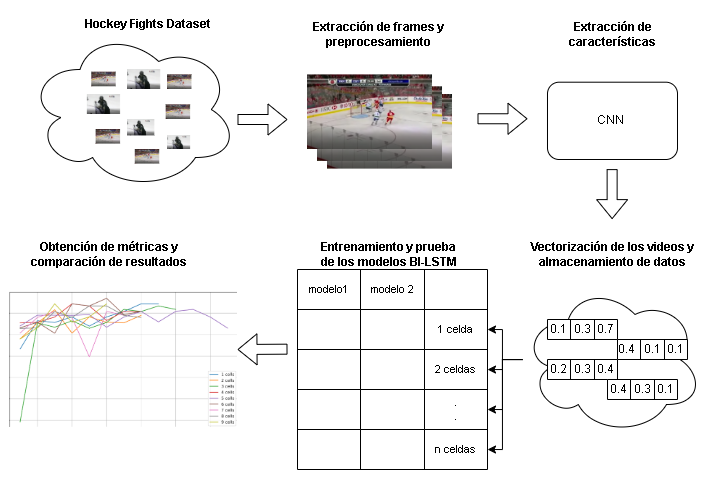
\includegraphics[width=0.7\textwidth]{images/metodologiaMaestria.png} 
    \centering 
    \caption{Metodología propuesta. Creación propia.} 
    \label{metodologia} 
\end{figure}

El \textit{pipeline} consiste en la obtencion, preprocesamiento 
y almacenamiento de las caracteristicas obtenidas del 
\textit{dataset}, para luego ser pasado a las diferentes 
configuraciones de los modelos BI-LSTM, los cuales se 
encargarán cada video basado en sus frames y finalmente 
se evaluarán los resultados basados en la métrica f1 y 
el tiempo de inferencia.

\subsection{Extracción de frames y preprocesamiento}

Como primer paso de la metodología se necesitó realizar un 
preprocesamiento de los datos para su análisis posterior a 
través de los modelos mencionados en el anterior capítulo. 
Como primer paso, se procedió a descargar el 
\textit{dataset} a través de su repositorio de 
\href{https://www.kaggle.com/datasets/yassershrief/hockey-fight-vidoes/data}{Kaggle}. \\

Una vez obtenidos los datos, se procedió a etiquetar cada uno 
de los videos basados en los nombres de cada uno de ellos. 
Se puede diferenciar su etiqueta debido a que aquellos que 
comiencen con "fi" contienen violencia, mientra que los demás, 
no. Con los videos cargados, se recolectaron los frames tal 
como fue mencionado anteriormente. Para ello, se decidió 
hacer un muestreo de 10 frames de manera equitativamente 
separada del video (1 por cada 4 frames). Cada uno de estos 
frames fueron redimensionados a un formato estandar (224 x 224) 
para luego ser normalizados.

\subsection{Obtención de las características}

Con cada conjunto de frames por video, estos pasan a través de 
las diferentes arquitecturas de CNN mencionadas en el anterior 
capítulo. Para ello, se tuvieron las siguientes consideraciones: 
\begin{itemize}
    \item Se obtendrán los modelos pre-entrenados con el 
    dataset ImageNet.
    \item Se eliminan las capas de clasificación.
    \item Se agrega una capa GlobalAveragePooling2D para 
    reducir la dimensionalidad de kernels(resultado de las CNN). 
    \item Se marca al modelo final como no entrenable.
\end{itemize}
 
Este ultimo paso es necesario debido a que se utilizará el 
conocimiento pre-entrenado de los modelos para obtener 
únicamente el vector característico de cada una de las 
imágenes. En ese sentido, se hace innecesario el proceso de 
entrenamiento de estas. Además, sería contraproducente tanto 
entrenar una CNN basado únicamente en frames porque pueden 
existir casos en el que existen frames donde no hay violencia 
y viceversa y también debido a que se perdería parte del 
conocimiento que ya tienen estos modelos. Finalemente se 
procedió a guardar estos vectores de características en 
formato h5. \\

Cabe resaltar que en la realidad podría implementarse un 
modelo conjunto con la CNN y LSTM, pero algunos de los modelos 
(especialmente los EfficientNet) contienen capas que no son 
facilmente mapeables a las entradas de las BI-LSTM, por lo 
cual se tuvo que hacer esto como  preprocesamiento.

\subsection{Entrenamiento y prueba del clasificador}

Como clasificador, se tuvo un modelo de BI-LSTM con diferente 
número de celdas. Para esta experimentación, se decidió usar 
un número entre 1 y 9 celdas, ya que consistía en un dataset 
bastante sencillo y altamente estudiado anteriormente. 

Para cada uno de las CNN's mencionadas en la anterior sección, 
y para cada una de las configuraciones, se procedió a 
entrenar y testear cada combinación de ellas. Las consideraciones 
para esta arquitectura fueron las siguientes:

\begin{itemize}
    \item De entrada se tienen los vectores de características 
    obtenidos del paso anterior (se debe considerar que los 
    tamaños de salida puden variar con respecto a la CNN). 
    \item Se crea un modelo BI-LSTM con X celdas, 10 timesteps 
    (en otras palabras los 10 frames obtenidos) y el tamaño 
    del output del anterior paso.
    \item Capas densas de 1024, 50 y 2 neuronas con funciones 
    de activación RelU y la última de tipo softmax. 
    \item Función de pérdida Binary CrossEntropy, optimizador adam 
    y de métricas accuracy y f1-score.
    \item Función de early stopping con \textit{patience} de 3 y  
    \textit{min delta} de 0.005 y batch de 16 videos por vez.
\end{itemize}

En la siguiente sección se presentarán los resultados 
generados utilizando las anteriores consideraciones para 
cada uno de los modelos mencionados.

\section{Experimentación}

Como primer paso, se procedió a realizar el pre-procesamiento 
de las imágenes y la obtención de sus características tal 
como fue mencionado anteriormente. Para ello, se recolectaron 
las métricas acerca de la cantidad de parámetros y el 
tiempo de cálculo de cada uno de los modelos, los cuales 
se puden observar en la Tabla \ref{tabla:procesamiento}:

\begin{table}[h!]
\centering
\begin{tabular}{|l|r|r|}
\hline
\multicolumn{1}{|c|}{\textbf{Modelo}} & \multicolumn{1}{c|}{\textbf{Parámetros}} & \multicolumn{1}{c|}{\textbf{\begin{tabular}[c]{@{}c@{}}Timpo de inferencia\\ (por batch de 10)\\ en ms/batch\end{tabular}}} \\ \hline
\textbf{efficientnetb0}               & 4,049,571                                & 46 ms                                                                                                                       \\ \hline
\textbf{resnet50}                     & 23,587,712                               & 51 ms                                                                                                                       \\ \hline
\textbf{efficientnetv2-s}             & 20,331,360                               & 75 ms                                                                                                                       \\ \hline
\textbf{MobilenetV3large}             & 2,996,352                                & 45 ms                                                                                                                       \\ \hline
\end{tabular}
\label{tabla:preprocesamiento}
\end{table}

Se puede apreciar que el tamaño final de los modelos fue 
menor que el esperado por la Tabla \ref{evaluacion}. 
Esto se debió a que no se están utilizando las capas densas 
de los modelos y se estan reemplazando con una capa 
GlobalAveragePooling2D, la cual obtiene el resultado del 
kernel final de las capas convolucioanles y las reduce a un 
solo resultado promediado. 

Habiendo obtenido las características de cada uno de las 
imágenes y los diez frames generados por cada uno de ellas, 
se entrenaron diferentes modelos BI-LSTM como fue mencionado 
anteriormente, teniendo desde 1 a 10 celdas para cada uno de 
los CNN utilizados. A continuación se muestran las gráficas 
de pérdida y f1 score para cada una de los experimentos. 

\begin{figure}[h!]
    \centering
    \subfloat[\centering F1 score por época]{\includegraphics[width=0.48\textwidth]{../graphs/efficientnetb0_val_loss_per_epoch.png}}
    \subfloat[\centering Pérdida por época]{\includegraphics[width=0.48\textwidth]{../graphs/efficientnetb0_val_f1_per_epoch.png}}\hfill
    \caption{Gráficos de pérdida y f1 score por época usando EfficientNetB0}
    \label{fig:combinedEfficientnetB0}
\end{figure}

Los gráficos de la figura \ref{fig:combinedEfficientnetB0} muestran 
un descenso de la pérdida generada de manera estable, en donde el 
clasificador con 1 capa se puede apreciar muy separado de las demás 
configuraciones. Fuera de ella, todas las demás configuraciones obtuvieron 
resultados muy similares. Sin embargo, se puede apreciar que la 
configuración con 4 celdas fue la que mejor resultado obtuvo en esa 
métrica. Algo muy similar se ve en la gráfica de f1 score. La configuración 
con una y dos celdas generaron peores resultados, mientras que las demás 
obtuvieron mejores resultados. La diferencia radica en que si consideramos 
el resultado final después de 8 épocas, la configuración con 9 celdas 
es la ganadora. Pero si se considera que el early stopping tenía una paciencia de 
3 épocas, tendríamos que considerar el resultado en la época 6, en donde la 
configuración con 7 celdas fue la que generó mejores resultados. 

\begin{figure}[h!]
    \centering
    \subfloat[\centering F1 score por época]{\includegraphics[width=0.48\textwidth]{../graphs/efficientnetv2-s_val_loss_per_epoch.png}}
    \subfloat[\centering Pérdida por época]{\includegraphics[width=0.48\textwidth]{../graphs/efficientnetv2-s_val_f1_per_epoch.png}}\hfill
    \caption{Gráficos de pérdida y f1 score por época usando EfficinetnetV2-S}
    \label{fig:combinedEfficientnetV2}
\end{figure}

A comparación de la anterior ejecución, los gráficos de la figura 
\ref{fig:combinedEfficientnetV2} muestran un descenso de la pérdida 
gerada menos estable. Los resultados no muestran un patrón único, por 
lo que la única conclusión basada en los datos es que los mejores resultados 
se obtuvieron con 2 y 5 celdas. Por otra parte, en términos de f1 score se 
pudo apreciar un mejor entrenamiento y resultado final en la configuración de 
2 celdas. 

\begin{figure}[h!]
    \centering
    \subfloat[\centering F1 score por época]{\includegraphics[width=0.48\textwidth]{../graphs/MobilenetV3large_val_loss_per_epoch.png}}
    \subfloat[\centering Pérdida por época]{\includegraphics[width=0.48\textwidth]{../graphs/MobilenetV3large_val_f1_per_epoch.png}}\hfill
    \caption{Gráficos de pérdida y f1 score por época usando MobilenetV3}
    \label{fig:MobilenetV3}
\end{figure}

Utilizando MobileNetV3 se obtuvo un patrón muy distintivo entre la 
gráfica de pérdida y f1 score. En ambos casos se tuvo un descenso de 
pérdida muy estables utilizando la configuración de una sola celda, 
mientras que las demás se comportaron muy erráticamente. Esto es 
probablemente debido a la configuración del modelo, ya que es uno de 
los más ligeros del estado del arte (y también de entre los utilizados 
para esta experimentación). En ese sentido, las configuraciones con 
múltiples celdas cayeron en un overfitting para los vectores de 
características salidos de la CNN, por ende generando valores negativos 
en ambas métricas. 

\begin{figure}[h!]
    \centering
    \subfloat[\centering F1 score por época]{\includegraphics[width=0.48\textwidth]{../graphs/resnet50_val_loss_per_epoch.png}}
    \subfloat[\centering Pérdida por época]{\includegraphics[width=0.48\textwidth]{../graphs/resnet50_val_f1_per_epoch.png}}\hfill
    \caption{Gráficos de pérdida y f1 score por época usando Resnet50}
    \label{fig:Resnet50}
\end{figure}

Las ejecuciones de Resnet50 generaron patrones más estables 
en ambos gráficos. En ese sentido la mayoría tuvo un descenso 
de la pérdida bastante similar entre ellos. Al compararlos 
teniendo en cuenta el early stopping, en la época 6 se 
generó una menor pérdida con el modelo de 6 épocas, lo cuál 
también concordó con ser el modelo con mejor f1 score de entre 
todos. Un dato interesante a analizar es el de la configuración 
con 7 celdas, el cual generó picos erráticos en el entrenamiento, 
lo cual también se reflejó en el gráfico de f1 score. Además, 
la configuración de 5 celdas tuvo una mayor cántidad de épocas 
de entrenamiento a comparación de los demás.

A continuación se muestran las métricas finales por cada uno de 
los modelos:

\begin{table}[h!]
\centering
\begin{tabular}{|l|l|l|l|l|l|l|}
\hline
\textbf{lstm\_cells} & \textbf{train\_loss} & \textbf{train\_f1} & \textbf{val\_loss} & \textbf{val\_f1} & \textbf{test\_loss} & \textbf{test\_f1} \\ \hline
\textbf{1}           & 0.0347               & 0.9873             & 0.2488             & 0.9408           & 0.0974              & 0.9725            \\ \hline
\textbf{2}           & 0.1213               & 0.9564             & 0.2392             & 0.9399           & 0.1674              & 0.9525            \\ \hline
\textbf{3}           & 0.0209               & 0.9902             & 0.1862             & 0.958            & 0.0698              & 0.9825            \\ \hline
\textbf{4}           & 0.047                & 0.9929             & \textbf{0.1038}    & 0.9541           & 0.1133              & 0.9575            \\ \hline
\textbf{5}           & 0.058                & 0.979              & 0.1506             & 0.9581           & 0.1049              & 0.97              \\ \hline
\textbf{6}           & 0.029                & 0.9931             & 0.1599             & 0.9541           & 0.0919              & 0.9725            \\ \hline
\textbf{7}           & 0.0258               & 0.9933             & 0.1367             & 0.9541           & 0.0691              & \textbf{0.985}    \\ \hline
\textbf{8}           & 0.0214               & 0.9929             & 0.2205             & 0.9412           & 0.1213              & 0.9625            \\ \hline
\textbf{9}           & \textbf{0.012}       & \textbf{0.9961}    & 0.1564             & \textbf{0.9667}  & \textbf{0.0605}     & \textbf{0.98}     \\ \hline
\end{tabular}
\caption{ Tabla comparativa de las métricas obtenidas por configuración de celdas para EfficientNetB0.}
\label{table:efficientnetb0Metrics}
\end{table}


En la tabla \ref{table:efficientnetb0Metrics} se las tienen 
métricas de pérdida y f1 score para todas las etapas: 
entrenamiento, validación y testeo para cada una de las 
configuraciones. En ella se puede ver que los mejores 
resultados de manera casi general fue la configuración de 9 
celdas, lo cual no se refleja con los resultados de validación 
que se vieron en los gráficos de pérdida y f1 score anteriormente 
mostrados. 


\begin{table}[h!]
\centering
\begin{tabular}{|l|l|l|l|l|l|l|}
\hline
\textbf{lstm\_cells} & \textbf{train\_loss} & \textbf{train\_f1} & \textbf{val\_loss} & \textbf{val\_f1} & \textbf{test\_loss} & \textbf{test\_f1} \\ \hline
\textbf{1}  & 0.0833               & 0.9693             & 0.2338             & 0.932            & 0.12                & 0.9675            \\ \hline
\textbf{2}  & 0.048                & 0.9869             & \textbf{0.1492}    & \textbf{0.9586}  & 0.0849              & 0.9775            \\ \hline
\textbf{3}  & 0.185                & 0.9349             & 0.3138             & 0.8779           & 0.2181              & 0.9175            \\ \hline
\textbf{4}  & 0.1111               & 0.9605             & 0.268              & 0.9187           & 0.1375              & 0.96              \\ \hline
\textbf{5}  & 0.0228               & 0.9936             & 0.1915             & 0.927            & 0.0666              & \textbf{0.9825}   \\ \hline
\textbf{6}  & 0.0396               & 0.9875             & 0.1626             & \textbf{0.9537}  & 0.0789              & \textbf{0.98}     \\ \hline
\textbf{7}  & 0.1473               & 0.9402             & 0.2269             & 0.932            & 0.1458              & 0.96              \\ \hline
\textbf{8}  & 0.0504               & 0.9872             & 0.1829             & 0.9139           & 0.1408              & 0.95              \\ \hline
\textbf{9}  & \textbf{0.018}       & \textbf{0.9969}    & 0.2741             & 0.9295           & \textbf{0.0649}     & \textbf{0.9825}   \\ \hline
\end{tabular}
\caption{ Tabla comparativa de las métricas obtenidas por configuración de celdas para EfficientnetV2.}
\label{table:efficientnetV2Metrics}
\end{table}

A comparación de la anterior tabla, utilizando los datos de la tabla 
\ref{table:efficientnetV2Metrics} no se puede sacar una conclusión 
específica acerca de cual configuración es la mejor a comparación del resto. 
Esto se puede ver debido a que los mejores resultados (obtenidos con 9 celdas) 
son diferentes para validación que para entrenamiento y testing. Además, 
al revisar los datos de los gráficos de validación mostrados anteriormente, se 
pudo ver que este estaba generando un ligero overfitting. 

\begin{table}[h!]
\centering
\begin{tabular}{|l|l|l|l|l|l|l|}
\hline
\textbf{lstm\_cells} & \textbf{train\_loss} & \textbf{train\_f1} & \textbf{val\_loss} & \textbf{val\_f1} & \textbf{test\_loss} & \textbf{test\_f1} \\ \hline
\textbf{1}           & 0.0562               & 0.9875             & \textbf{0.1048}    & \textbf{0.9716}  & \textbf{0.0721}     & \textbf{0.9825}   \\ \hline
\textbf{2}           & 0.0527               & 0.9845             & 0.2139             & 0.9287           & 0.1006              & 0.9775            \\ \hline
\textbf{3}           & \textbf{0.0237}      & \textbf{0.9969}    & 0.1774             & 0.9408           & 0.1117              & 0.965             \\ \hline
\textbf{4}           & 0.092                & 0.9655             & 0.2456             & 0.8904           & 0.1914              & 0.935             \\ \hline
\textbf{5}           & 0.1141               & 0.9649             & 0.3142             & 0.9295           & 0.1982              & 0.9325            \\ \hline
\textbf{6}           & 0.0376               & 0.987              & 0.2237             & 0.9283           & 0.1158              & 0.97              \\ \hline
\textbf{7}           & 0.0376               & 0.986              & 0.1745             & 0.9537           & \textbf{0.0706}     & 0.9775            \\ \hline
\textbf{8}           & 0.0497               & 0.986              & 0.186              & 0.9413           & 0.1219              & 0.965             \\ \hline
\textbf{9}           & 0.0807               & 0.9772             & 0.1777             & 0.9282           & 0.1368              & 0.9625            \\ \hline
\end{tabular}
\caption{ Tabla comparativa de las métricas obtenidas por configuración de celdas para MobileNetV3.}
\label{table:MobileNetV3Metrics}
\end{table}

La tabla \ref{table:MobileNetV3Metrics} muestra resultados más 
concluyentes a comparación de las demás. Al igual que con los gráficos 
anteriores, se puede ver que si bien no se obtuvieron los mejores 
resultados finales para entrenamiento, si lo hizo para prueba y testeo. 
Además, se puede ver que estos empeoran mientras más celdas de BI-LSTM 
se usan. En ese sentido, se puede afirmar que esta es la mejor 
configuración para este modelo, 

\begin{table}[h!]
\centering
\begin{tabular}{|l|l|l|l|l|l|l|}
\hline
\textbf{lstm\_cells} & \textbf{train\_loss} & \textbf{train\_f1} & \textbf{val\_loss} & \textbf{val\_f1} & \textbf{test\_loss} & \textbf{test\_f1} \\ \hline
\textbf{1}           & 0.1039               & 0.9769             & 0.1382             & \textbf{0.9716}  & 0.116               & 0.9725            \\ \hline
\textbf{2}           & 0.0907               & 0.9808             & 0.2067             & 0.9448           & 0.1111              & 0.97              \\ \hline
\textbf{3}           & 0.0837               & 0.9771             & \textbf{0.1177}    & 0.9586           & 0.1183              & 0.9675            \\ \hline
\textbf{4}           & \textbf{0.0471}      & \textbf{0.9904}    & 0.1298             & 0.9537           & \textbf{0.0858}     & \textbf{0.98}     \\ \hline
\textbf{5}           & \textbf{0.049}       & \textbf{0.993}     & 0.1499             & 0.9148           & \textbf{0.0866}     & \textbf{0.9775}   \\ \hline
\textbf{6}           & 0.0925               & 0.9649             & 0.1553             & 0.9541           & 0.0973              & 0.975             \\ \hline
\textbf{7}           & 0.1106               & 0.9551             & 0.18               & 0.9448           & 0.1374              & 0.9525            \\ \hline
\textbf{8}           & 0.1262               & 0.9576             & 0.1257             & 0.9399           & 0.1074              & 0.975             \\ \hline
\textbf{9}           & 0.0624               & 0.9872             & 0.1742             & \textbf{0.9716}  & 0.1188              & 0.97              \\ \hline
\end{tabular}
\caption{ Tabla comparativa de las métricas obtenidas por configuración de celdas para Resnet50.}
\label{table:Resnet50}
\end{table}

Observando los datos de la tabla \ref{table:Resnet50} es 
notorio que los mejores resultados estuvieron en las 
configuraciones medias (4 y 5 celdas). Además también se 
logra idntificar que mientras más o menos celdas, todas las 
métricas se reducen, salvo con el caso de 9 celdas, el cual 
es un dato anómalo en esa distribución. 

Por último, a continuación se mostrará una tabla comparativa 
resumen de toda la experimentación realizada en el presente trabajo: 

\begin{table}[h!]
\centering
\begin{tabular}{|l|l|l|l|l|l|l|l|}
\hline
\textbf{cnn\_model}     & \textbf{lstm\_cells} & \textbf{train\_loss} & \textbf{train\_f1} & \textbf{val\_loss} & \textbf{val\_f1} & \textbf{test\_loss} & \textbf{test\_f1} \\ \hline
\textbf{EfficientNetB0} & 9                    & \textbf{0.012}       & \textbf{0.9961}    & 0.1564             & \textbf{0.9716}  & \textbf{0.0605}     & \textbf{0.98}     \\ \hline
\textbf{EfficientNetV2} & 9                    & 0.018                & \textbf{0.9969}    & 0.2741             & 0.9295           & \textbf{0.0649}     & \textbf{0.9825}   \\ \hline
\textbf{MobileNetV3}    & 1                    & 0.0562               & 0.9875             & \textbf{0.1048}    & \textbf{0.9716}  & 0.0721              & \textbf{0.9825}   \\ \hline
\textbf{ResNet50}       & 4                    & 0.0471               & 0.9904             & 0.1298             & 0.9537           & 0.0858              & \textbf{0.98}     \\ \hline
\end{tabular}
\caption{ Tabla comparativa resumen final de la experimentación}
\label{table:Resnet50}
\end{table}

Con los resultados finales se puede corroborar que todas las 
combinaciones entre CNN y LSTM lograron valores similares para 
todas las métricas de testeo al tener un f1 score . En ese sentido, 
y con el fin de optimizar el \textit{pipeline} final para el 
\textit{dataset} propuesto, sería recomendable utilizar MobileNetV3 
con una celda LSTM, ya que proporcionó el mismo resultado pero tanto 
el peso del modelo como el número de celdas es menor que en todas las 
demás configuraciones.


\chapter{Conclusiones y Trabajo Futuro}

En la Ecuación \eqref{eq:eq1secCTF}


\begin{equation}\label{eq:eq1secCTF}
M=\begin{pmatrix}
	m_{11}&m_{12}\\
	m_{21}&m_{22}
\end{pmatrix}
\end{equation}

En la siguiente Tabla \ref{tab:tab1secCTF}

\begin{table}[h]
\centering
\begin{tabular}{|c|c|}
	\hline
	1 & 2 \\
	\hline
	22 & 11 \\
	\hline
\end{tabular}
\caption{Tabla 1}
\label{tab:tab1secCTF}
\end{table}

En la siguiente Figura \ref{fig:fig1secCTF}

\begin{figure}[h]
\includegraphics[width= 0.8\textwidth]{logo_unir}
\caption{Logo Unir}
\label{fig:fig1secCTF}
\end{figure}

\cite{PIMENTEL2016744} \cite{da_S_Bessa_2023}


%\begin{thebibliography}{a}
%\bibitem{etiqueta} \textsc{Autores},
%\textit{nombre referencia.}
%Información addicional
%\end{thebibliography}
\bibliographystyle{apacite}
\bibliography{bibliografia}

\appendix
\chapter{Apendices}

\end{document}





















